\subsection{Arquitectura funcional}
De acuerdo con los requerimientos definidos en la etapa anterior, se pueden enumerar las funciones necesarias los procesos del sistema. Estas se pueden dividir en varias subfunciones para visualizar mejor cada uno de los procesos que se llevarán a cabo dentro del dispositivo. Estas funciones se pueden ver de forma jerárquica en la figura \ref{fg:Funciones} y también es posible observar su interrelación en el diagrama IDEF-0 que se muestra en la figura \ref{fg:IDEFGeneral}. Con mayor detalle, puede revisar el apéndice \ref{Ap:IDEF0}.

0. Función Principal: \textbf{Generar compost }
\begin{itemize}
    \item 1. Recepción de la materia
    \begin{itemize}
        \item 1.1 Triturar la materia a la entrada
        \item 1.2 Conducir la materia al interior del contenedor
        \begin{itemize}
            \item 1.2.1. Empujar la materia al interior
            \item 1.2.2. Almacenar la materia
        \end{itemize}
    \end{itemize}
    \item 2. Regular las diferentes etapas del proceso de compostaje
    \begin{itemize}
        \item 2.1. Gestionar el periodo de tiempo para cada fase
        \begin{itemize}
            \item 2.1.1. Contar horas, minutos y segundos.
            \item 2.1.2 Delimitar cada periodo de inicio y final en cada etapa del proceso.
        \end{itemize}
        \item 2.2. Regular la temperatura en cada fase de manera automática.
        \begin{itemize}
            \item 2.2.1 Monitorear el valor de la temperatura
            \item 2.2.2 En caso de una temperatura inferior, encender los actuadores necesarios para incrementar la temperatura de la materia.
            \item 2.2.3 En caso de una temperatura superior, encender los actuadores necesarios para disminuir la temperatura
            \item 2.2.4 Conservar una temperatura constante al interior del contenedor.
            \begin{itemize}
                \item 2.2.4.1 Reducir las pérdidas de calor.
                \item 2.2.4.2 Contar con un cierre firme para evitar las fugas de materia orgánica.
            \end{itemize}
        \end{itemize}
    \end{itemize}
    \item 3. Gestionar los tiempos del proceso de aireación
    \begin{itemize}
        \item 3.1. Contar el tiempo para activar cada ciclo de aireación.
        \item 3.2. Activar de manera automática cada uno de los actuadores para el proceso de aireación.
    \end{itemize}
    \item 4. Gestionar la comunicación con el usuario
    \begin{itemize}
        \item 4.1. Mantener una comunicación bidireccional por medio de una interfaz humano-maquina
        \begin{itemize}
            \item 4.1.1. Enviar información del proceso
            \begin{itemize}
                \item 4.1.1.1. Enviar información sobre el ambiente al interior del contenedor
                \item 4.1.1.2. Enviar información sobre que proceso se esta ejecutando
                \item 4.1.1.3. Enviar información sobre el tiempo total del proceso.
            \end{itemize}
            \item 4.1.2. Recibir indicaciones para activar los diferentes actuadores un modo de prueba.
        \end{itemize}
        \item 4.2. Mantener una comunicación unidireccional a través de un sitio web.
        \begin{itemize}
            \item 4.2.1 Enviar información sobre las variables ambientales al interior del contenedor
            \item 4.2.2. Enviar información sobre que actuadores están activos.
            \item 4.2.3. Enviar información sobre el tiempo total del proceso.
        \end{itemize}
    \end{itemize}
\end{itemize}

\begin{figure}[h!]
            \centering
            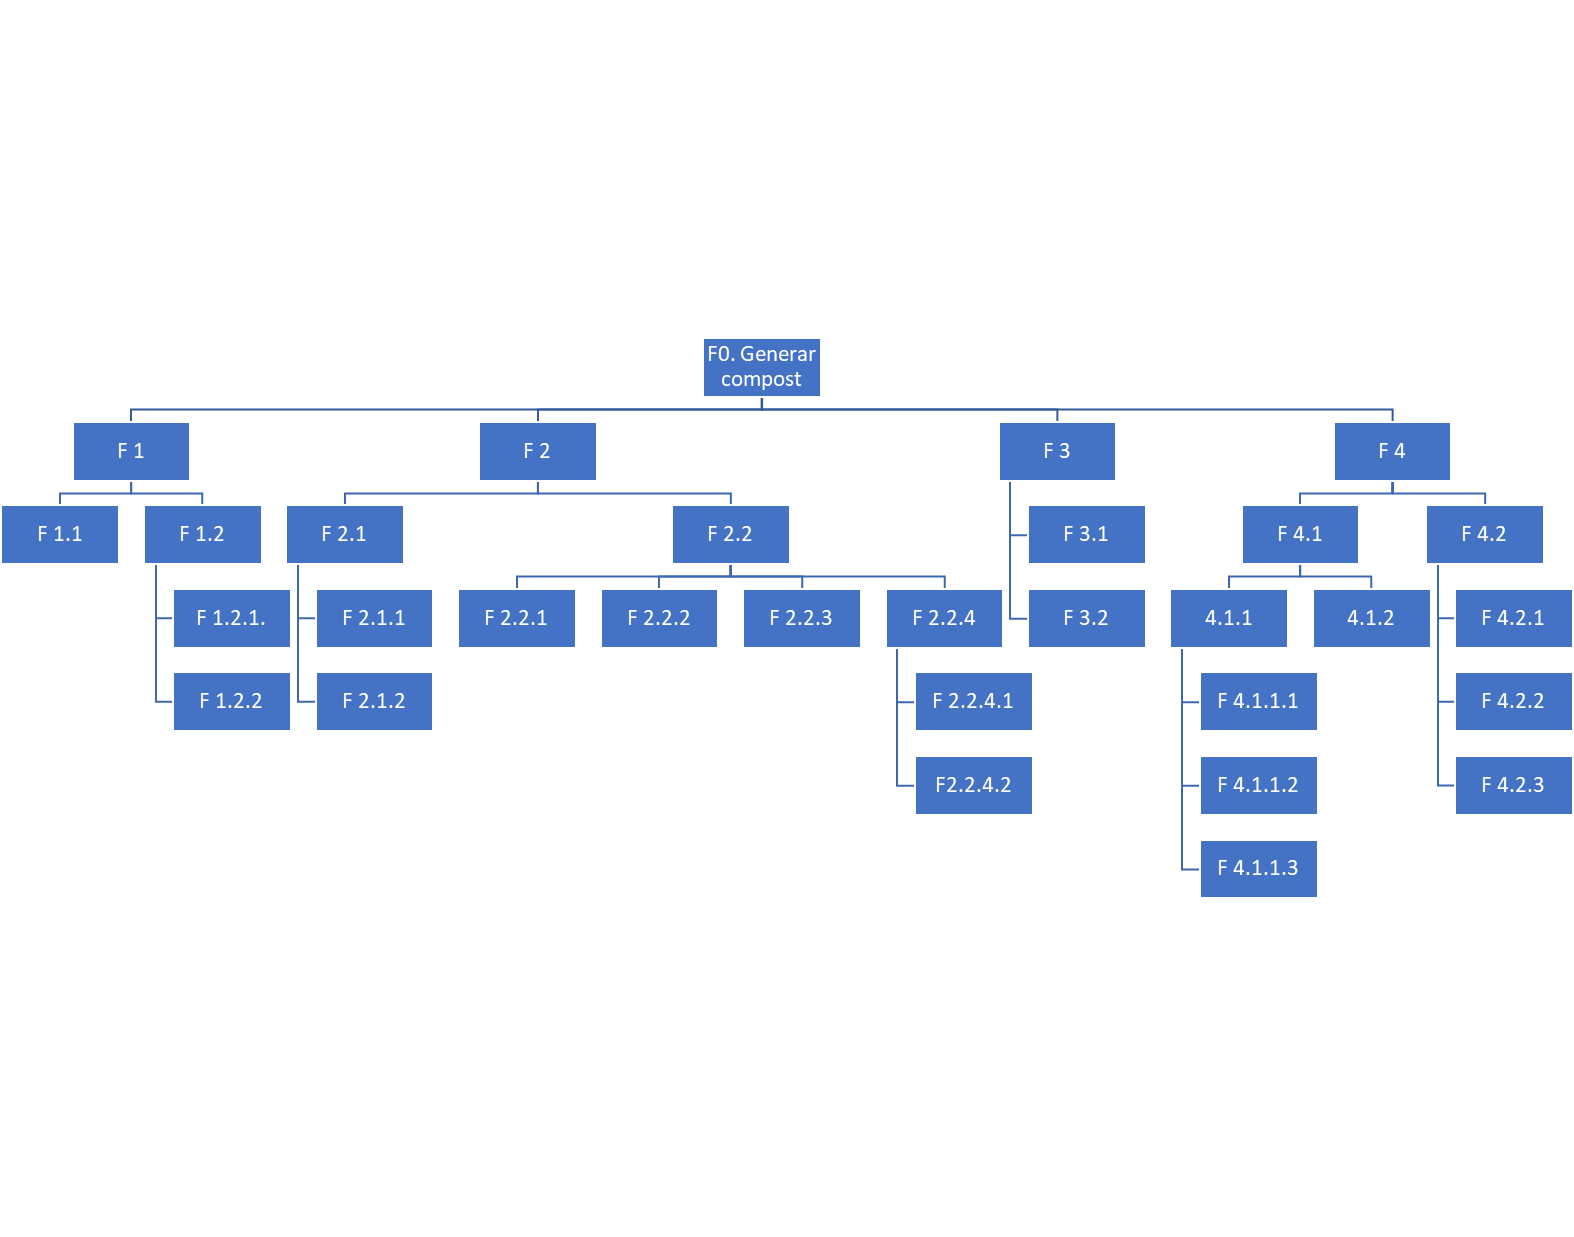
\includegraphics[scale=0.3, angle = 90]{images/Capitulo 3/3.1.1.2 Arquitectura funcional/FBS2.png}
            \caption{Diagrama FBS del sistema}
            \label{fg:Funciones}
        \end{figure}

\newpage

\begin{figure}[h!]
            \centering
            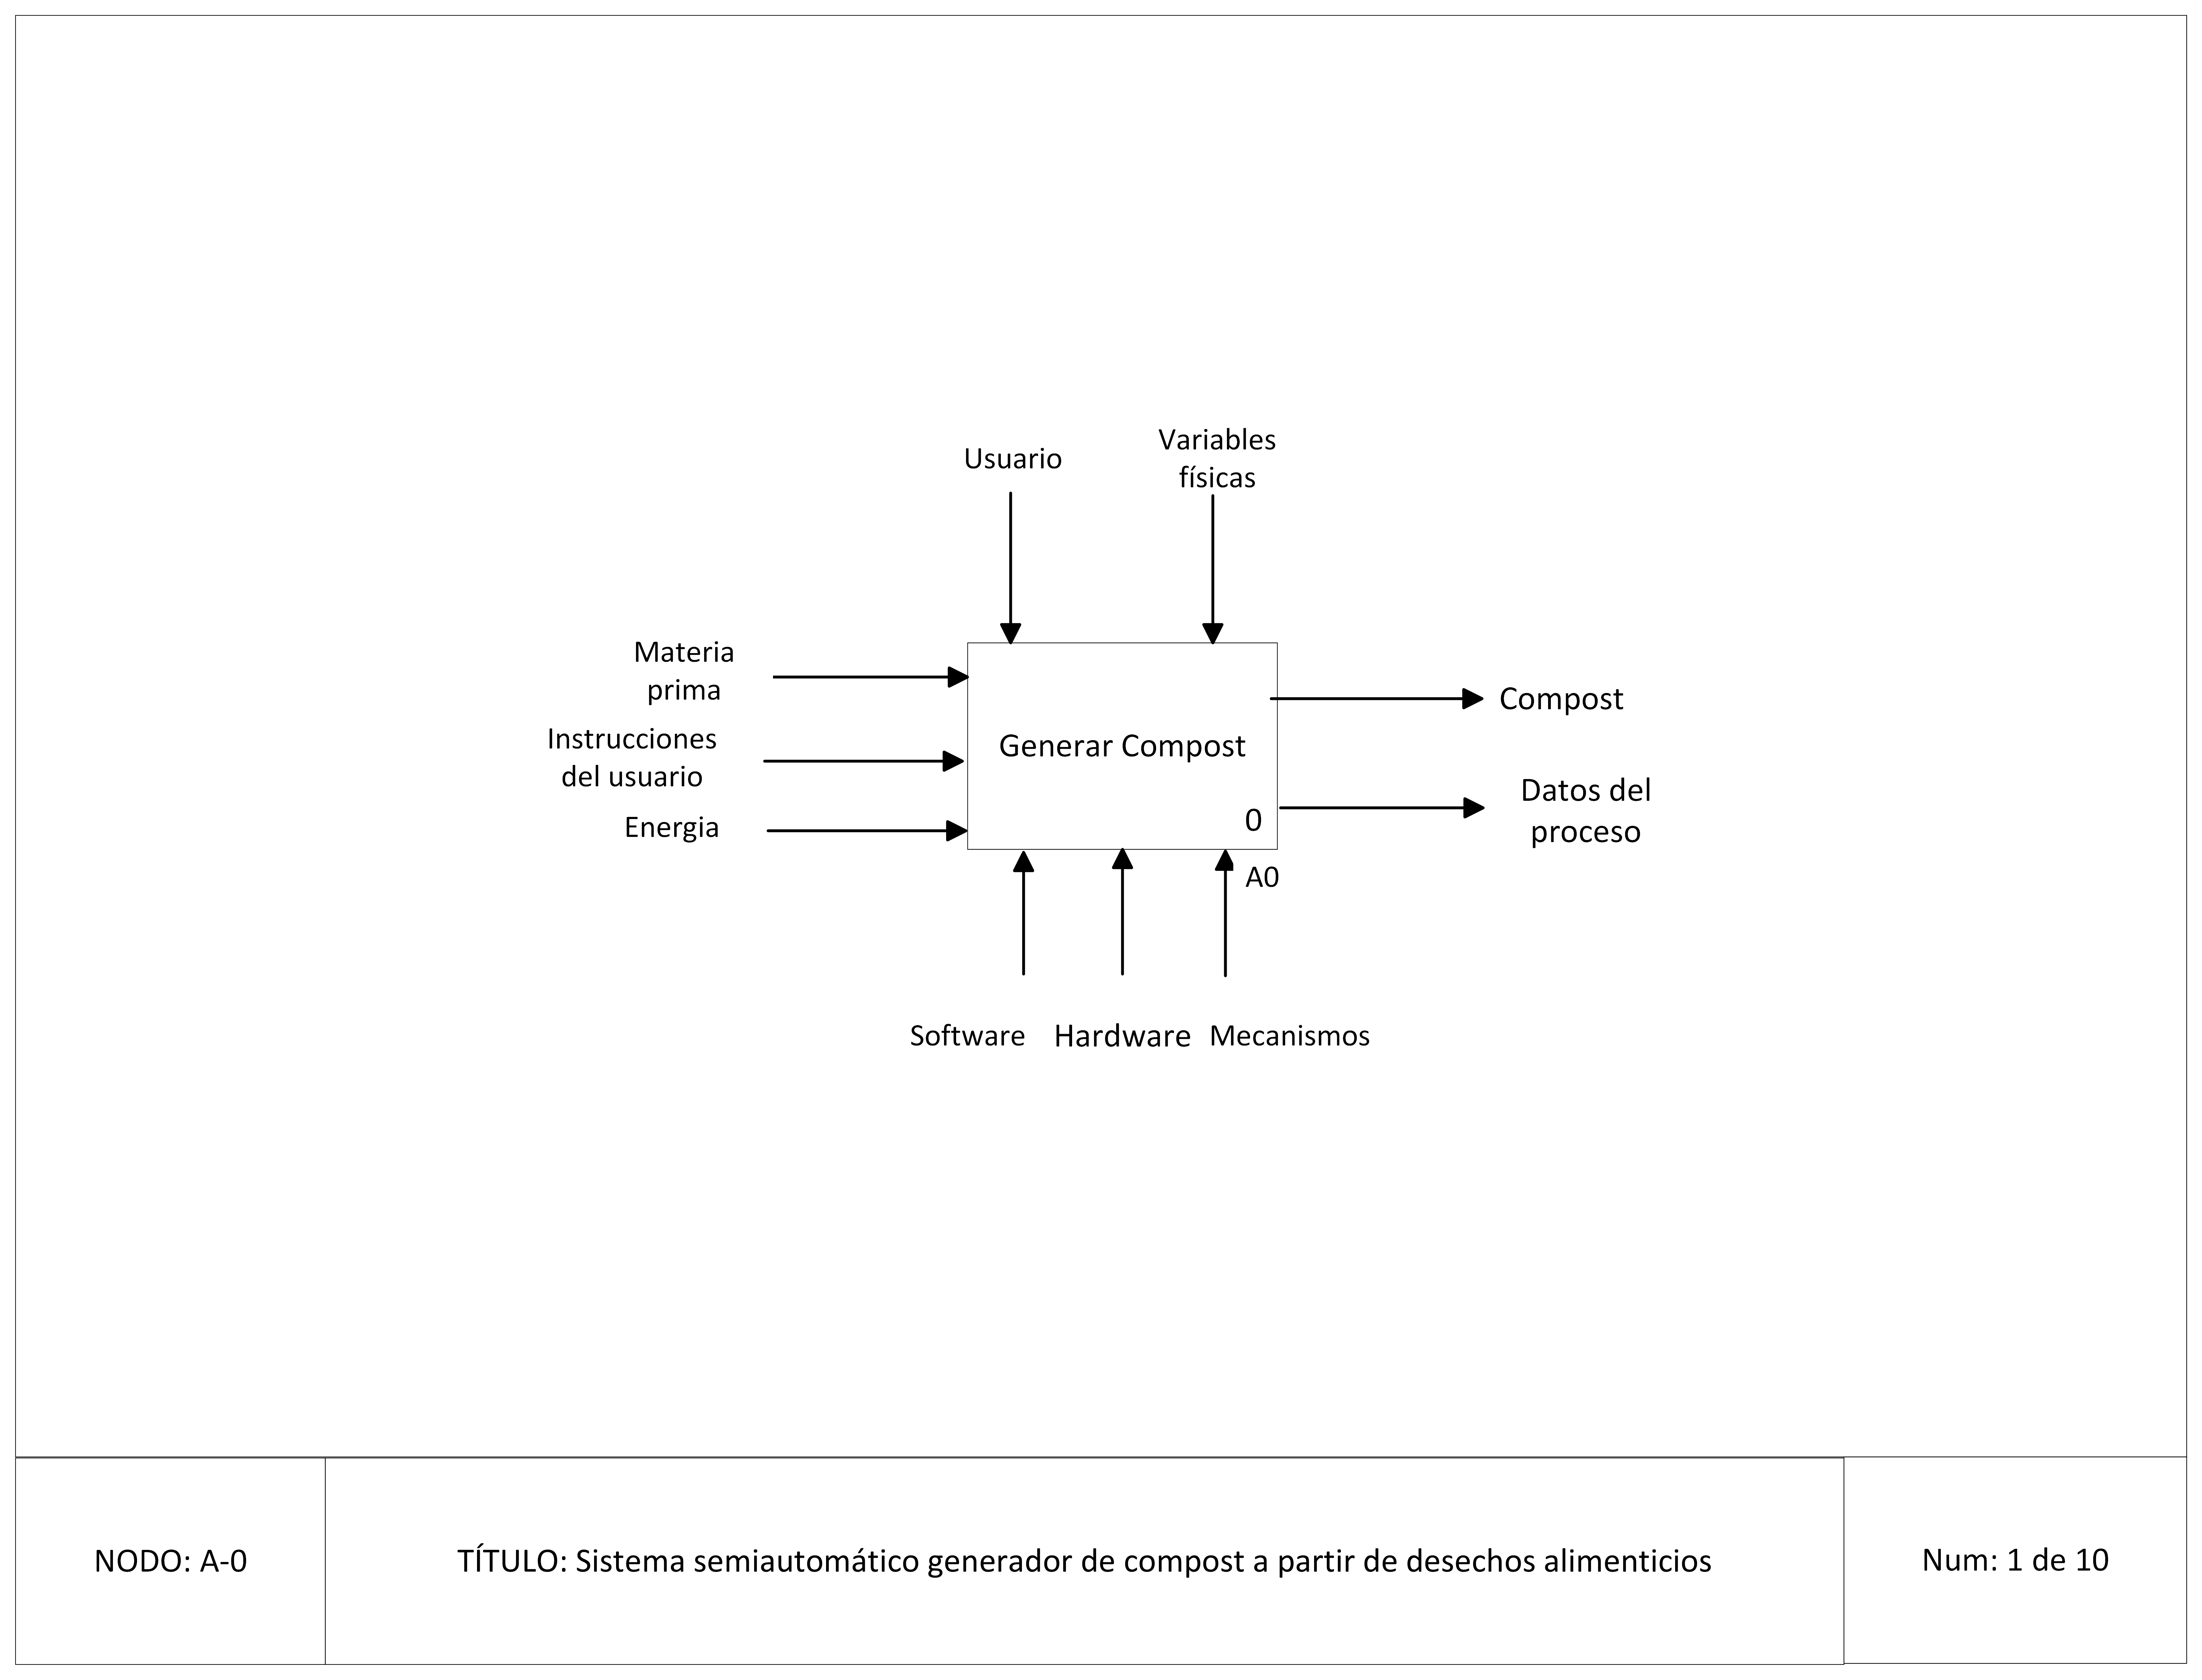
\includegraphics[scale=0.2, angle = 90]{images/Capitulo 6 Apéndices/01 IDEF 0/General.png}
            \caption{IDEF0 del sistema}
            \label{fg:IDEFGeneral}
\end{figure}

\newpage        
Una vez que se han descrito las entradas y las salidas requeridas del sistema, es necesario detallar cómo es que se interrelacionan las diferentes funciones en su interior. En la figura \ref{fg:IDEFA0} se presenta el Nodo: A0 expandido, mostrando de forma detallada la función \textbf{Generación de compost}.

\begin{figure}[h!]
    \centering
    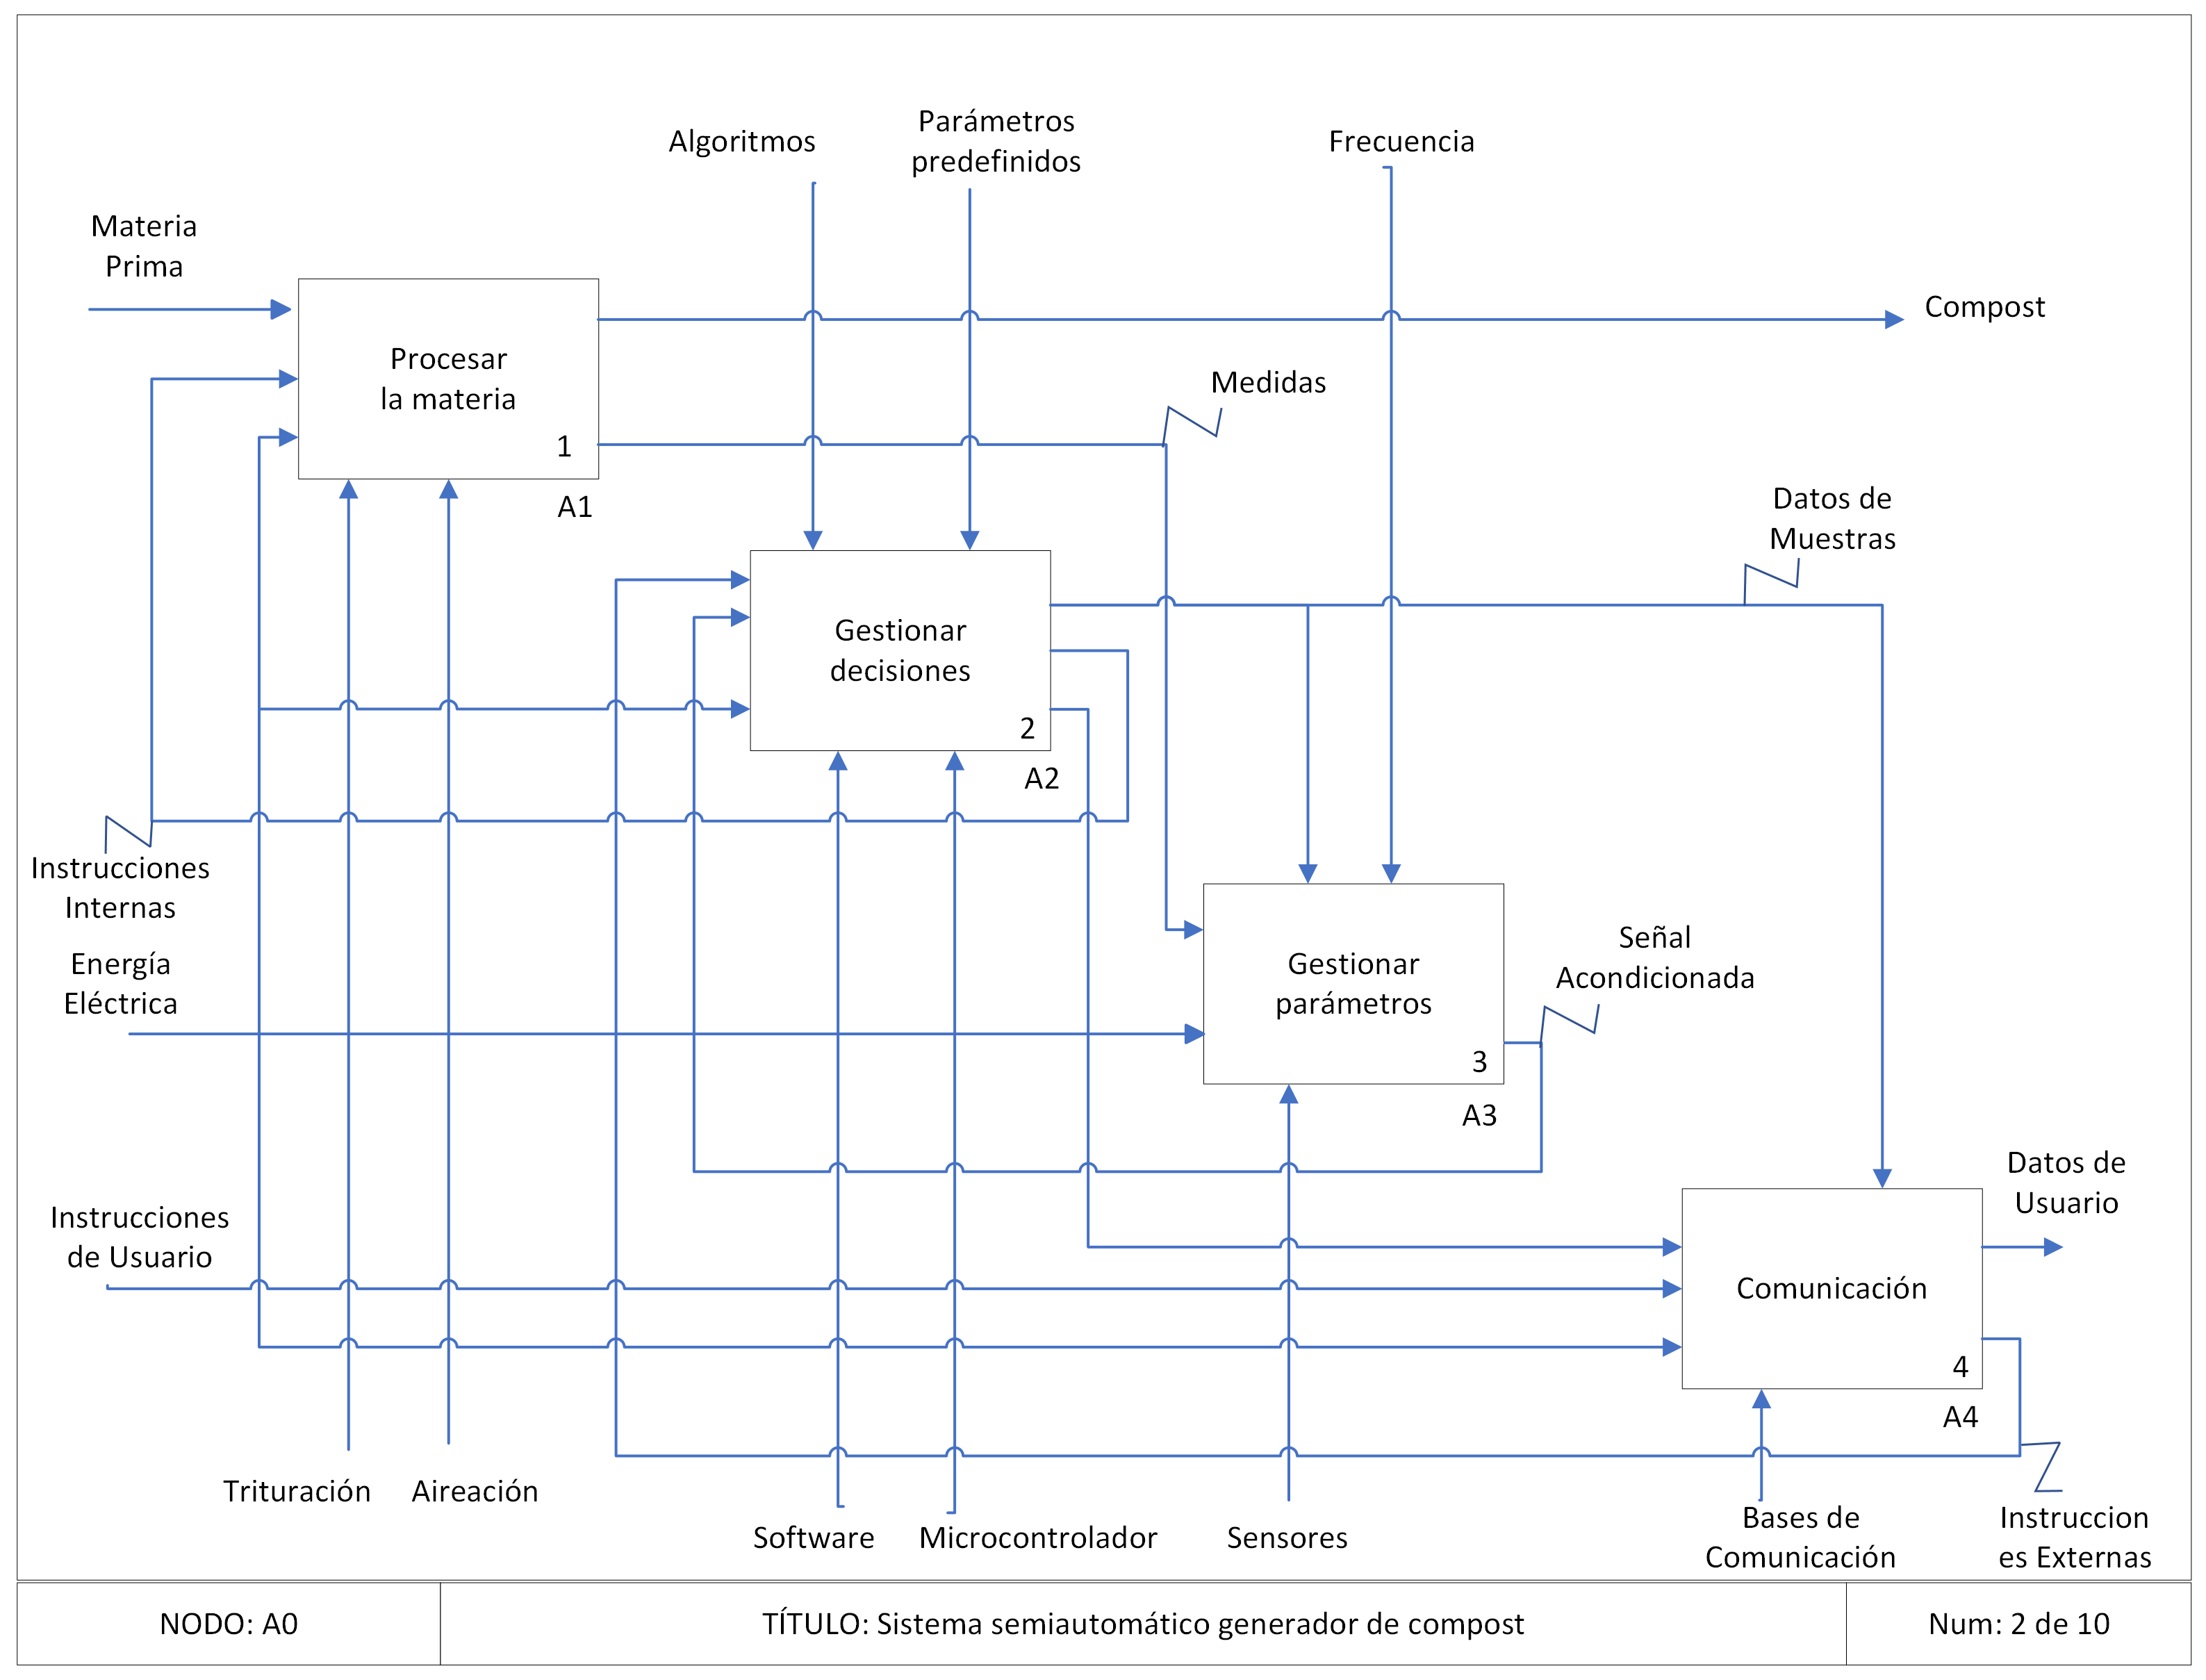
\includegraphics[scale=0.2, angle = 90]{images/Capitulo 6 Apéndices/01 IDEF 0/NodoA0.png}
    \caption{IDEF0 Nodo: A0}
    \label{fg:IDEFA0}
\end{figure}

De esta forma, se puede observar cómo se describen las funciones principales del sistema, a partir de las entradas principales: \textbf{Materias primas}, \textbf{Instrucciones del usuario} y \textbf{Energía eléctrica}. 

El sistema será capaz de proveer a la salida \textbf{Compost}, además de entregar \textbf{Datos al usuario} sobre el estado de las variables físicas internas del dispositivo e información sobre el proceso de compostaje. Para poder obtener las salidas deseadas del sistema, es necesario que los procesos y las funciones principales estén controladas por diversas herramientas, como lo son \textbf{Algoritmos de programación}, \textbf{Los parámetros predefinidos}, \textbf{Instrucciones de usuario}, así como \textbf{Señales de comunicación internas} las cuales son necesarias para coordinar la operaciones y las etapas de cada uno de los procesos requeridos para generar el ambiente que beneficie los procesos de descomposición. 


